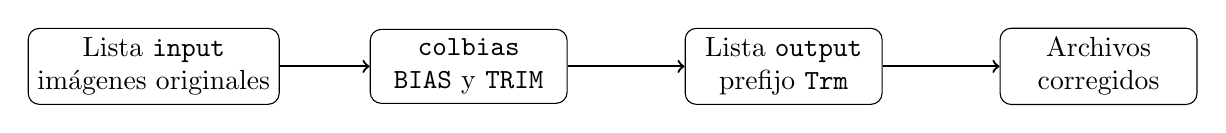
\begin{tikzpicture}[
  box/.style={draw,rounded corners,align=center,minimum width=2.5cm,minimum height=0.85cm},
  arrow/.style={->,thick}
]
  \node[box] (input) at (0,0) {Lista \texttt{input}\\imágenes originales};
  \node[box] (task) at (4,0) {\texttt{colbias}\\\texttt{BIAS} y \texttt{TRIM}};
  \node[box] (output) at (8,0) {Lista \texttt{output}\\prefijo \texttt{Trm}};
  \node[box] (images) at (12,0) {Archivos\\corregidos};
  \draw[arrow] (input) -- (task);
  \draw[arrow] (task) -- (output);
  \draw[arrow] (output) -- (images);
\end{tikzpicture}